\section{Validation}
\label{sec:validation}
\begin{itemize}
	\item By relying on \moccml, the application of \bcool operators generates a coordination specification in \ccsl. We can then use \ccsl tool (TimeSquare~\cite{timesquarebib}) to perform analyze and execute the generated coordination specification. 
	
	\item \todo{To show \ccsl code}
	
	\item To validate the coordinated, we provide two methods: execution and state-space exploration. 
	
	\item The state space exploration only valid when models has a finite execution. 
	
	\item In this section, we show the possible validation and verification activities that we can perform on the coordinated system. 
	
	\item By using TimeSquare, we can execute the coordinated system. Figure~\ref{?} illustrates the partial timing output of the execution of the whole example.
	
	\item Before be coordinated, FSMEvents and Action are allowed to occur, individual semantics makes their own choices. The coordination constrains the occurences of these events thus reducing what can be done by individual models. For instance,     

	\begin{figure}[h]
		\center
		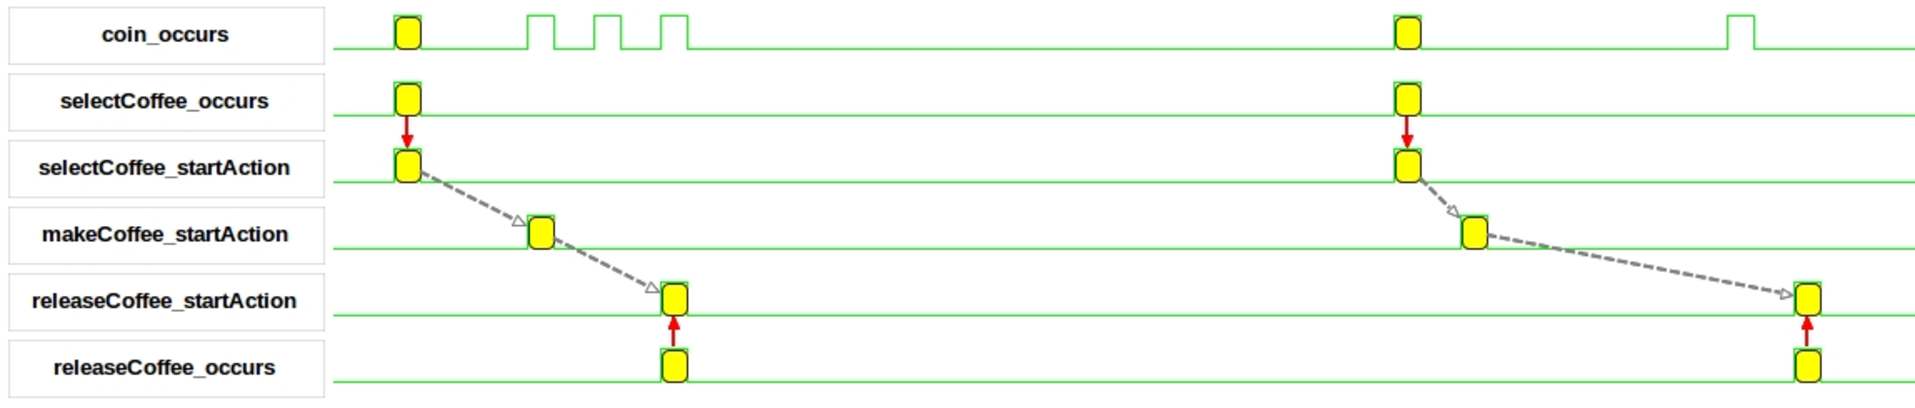
\includegraphics[width=.9\textwidth]{bcool/figs/coffeemachinevcd}
		\caption{todo}
		\label{fig:runningeventvar}
	\end{figure}
	
	\item The workbench also offers the possibility to obtain by exploration quantitative results on the scheduling state-space.
	
	\item \todo{To describe a bit the execution}
	\item . Then, the coordination constrains such events thus limiting the behavior of both models. Since the constrains expressed by the coordination these events becomes precedes. The simulation then only will the scenario where these events are precedes. 
	
	\item The semantics of Activity allows the multiple execution of the activity, however, given the constrain imposed by the coordination, the execution is controlled by the TFSM. 
	
	\item \todo{To describe how the behavior of both models is contraint by the glue. The global behavior is intersecction of both behaviors}
	
\end{itemize}